%
% File eacl2017.tex
%
%% Based on the style files for ACL-2016
%% Based on the style files for ACL-2015, with some improvements
%%  taken from the NAACL-2016 style
%% Based on the style files for ACL-2014, which were, in turn,
%% Based on the style files for ACL-2013, which were, in turn,
%% Based on the style files for ACL-2012, which were, in turn,
%% based on the style files for ACL-2011, which were, in turn, 
%% based on the style files for ACL-2010, which were, in turn, 
%% based on the style files for ACL-IJCNLP-2009, which were, in turn,
%% based on the style files for EACL-2009 and IJCNLP-2008...

%% Based on the style files for EACL 2006 by 
%%e.agirre@ehu.es or Sergi.Balari@uab.es
%% and that of ACL 08 by Joakim Nivre and Noah Smith

\documentclass[11pt]{article}
\usepackage{eacl2017}
\usepackage{times}
\usepackage{url}
\usepackage{xspace}
\usepackage{latexsym}
\usepackage[pdftex]{graphicx}

\def \eg {e.g.,\@ }
\def \ie {i.e.,\@ }
\def \al {al.\@ }
\def \etc {etc.\@ }

%\eaclfinalcopy % Uncomment this line for the final submission
%\def\eaclpaperid{***} %  Enter the acl Paper ID here

%\setlength\titlebox{5cm}
% You can expand the titlebox if you need extra space
% to show all the authors. Please do not make the titlebox
% smaller than 5cm (the original size); we will check this
% in the camera-ready version and ask you to change it back.

\newcommand\BibTeX{B{\sc ib}\TeX}

% TJB macros
\newcommand{\dotts}{...}
\newcommand{\gap}{$*$\xspace}
\newcommand{\ex}[1]{\textit{#1}\xspace}
\newcommand{\termdef}[1]{\textbf{#1}\xspace}
\newcommand{\termemph}[1]{\textit{#1}\xspace}

\newcommand{\figref}[2][]{Figure#1~\ref{#2}\xspace}
\newcommand{\tabref}[2][]{Table#1~\ref{#2}\xspace}
\newcommand{\secref}[2][]{Section#1~\ref{#2}\xspace}



\title{Unsupervised Acquisition of Comprehensive Multiword Lexicons \\ using Competition in an $n$-gram Lattice}

\author{First Author \\
  Affiliation / Address line 1 \\
  Affiliation / Address line 2 \\
  Affiliation / Address line 3 \\
  {\tt email@domain} \\\And
  Second Author \\
  Affiliation / Address line 1 \\
  Affiliation / Address line 2 \\
  Affiliation / Address line 3 \\
  {\tt email@domain} \\}

\date{}

\begin{document}
\maketitle
\begin{abstract}

\end{abstract}

\section{Introduction}

\section{Background and Related Work}

In this paper we will refer to the targets of lexicon creation efforts as \termdef{formulaic sequences}, following the terminology of Wray \shortcite{Wray02,Wray08}, wherein a formulaic sequence (FS) is defined as ``a sequence, continuous or discontinuous, of words or other elements, which is, or appears to be, prefabricated: that is, stored and retrieved whole from memory at the time of use, rather than being subject to generation or analysis by the language grammar.'' In other words, a formulaic sequence shows signs of being part of a mental lexicon. Though by this definition single individuals or small groups may have their own FS, in this paper, we are only interested in FS that are shared by a recognizable language community. In computational linguistics, the most common term used to describe multiword lexical units is \emph{multiword expression} or ``MWE'' \cite{Sag02,Baldwin10}, but here we wish to make a principled distinction between at least somewhat non-compositional, strongly lexicalized MWEs and FS, a near superset which includes most MWEs but also (apparently) compositional linguistic formulas. This distinction is not a new one; it exists, for example, in the original paper of \newcite{Sag02} in the distinction between lexicalized and institutionalized phrases, and also to some extent in the MWE annotation of \newcite{Schneider14a}, who distinguish between weak (collocational)\footnote{Here we avoid the term \emph{collocation} entirely due to even more confusion with respect to in its interpretation. Though in some contexts it has been used in way that is similar to our definition of FS, it can be applied to any words that show a statistical tendency to appear in the vicinity of one another for any reason: for instance, the pair of words \ex{doctor/nurse} might be considered a collocation \cite{Ramisch14}}  and strong (non-compositional) MWEs. It is our contention, however, that separate, precise terminology is useful for research targeted at either class: we need not strain the concept of MWE to include items which do not require special semantics, nor are we inclined to disregard the larger formulaticity of language simply because it is not the dominant focus of MWE research. Many MWE researchers would defensibly balk at including in their MWE lexicons and corpus annotations (English) formulaic sequences such as \ex{there is something going on}, \ex{it is more important than ever to \dotts}, \ex{\dotts do not know what it is like to \dotts}, \ex{there is no shortage of\dotts}, \ex{the rise and fall of\dotts}, \ex{now is not the time to\dotts}, \etc as well as tens of thousands of other such phrases which, along with less compositional MWEs like \ex{be worth \gap weight in gold}, fall under the FS umbrella. Another reason to consider a different terminology is that there are classes of what is typically considered MWE that don't fit well into an FS framework, for instance novel compound nouns whose semantics are accessible by analogy (\eg \ex{plastic house}). Also, we exclude from the definition of both FS and MWE those named entities which refer to people or places which are little-known and/or whose surface form appears derived (\eg \ex{Mrs. Barbara W. Smith} or \ex{Smith Garden Supplies Ltd}). \figref{fig:terminology} show the conception of the relationship between FS, MWE and (multiword) named entities that we assume for this paper.


\begin{figure}[!t]
\center{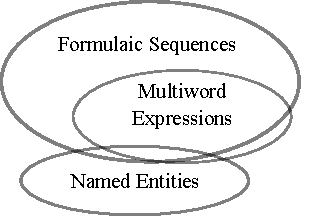
\includegraphics[width=0.35\textwidth]{FS_diagram_1.pdf}}
\caption{Multiword Terminology}
\label{fig:terminology}
\end{figure}



%We use the term \termdef{collocation} to refer to statistical co-occurrence without necessarily any lexicalization of the sort implied by our definition of FS. 
% TJB: I'd suggest staying away from talking about collocations altogether: it's an overloaded term; many MWEs are *not* collocations under this definition; and it's not needed for this paper
%MWEs are a non-compositional subset of FS, and they overlap with named entities (NEs). In this regard, we disagree with the MWE annotation schema of \newcite{Schneider14a} which includes any NE as an MWE, which, in the context of product reviews from the Web Treebank, means that that named entities form nearly 50\% of the MWEs types attested in that corpus, with many being phrases such as \ex{Tintman Nationwide Tints Ltd} or \ex{Hickory Furniture Mart} which are easily identifiable as NEs based on their form, but would not be considered part of the mental lexicon of even a tiny fraction of English speakers.% (not even, we might argue, most of these people who work for these businesses, they likely refer to them using shorter, informal names). 
% TJB: too subtle/controversial a point for this paper
%The upshot of this choice that a significant portion of ``MWE'' identification in the dataset is in fact named entity recognition. Some well-known named entities are obviously good MWEs (\eg \ex{George Washington}, \ex{the United States}), but not the names of the vast majority of people, businesses, or products which have real-word referents; they do not belong in a lexicon of formulaic sequences which is intended to reflect the internal lexicon of (at least) a significant generalizable subset of English speakers, putting them outside the scope of this work.

Regardless of the terminology used to describe them, the starting point for multiword lexicon creation has been typically lexical association measures \cite{Church90,Dunning93,Schone01,Evert04,Pecina10,DeAraujo11,Kulkarni11,Ramisch14}; when these methods are used to build a lexicon, particular syntactic patterns and thresholds for the metrics are typically chosen. Only some of these measures generalize tractably beyond two words, for example PMI \cite{Church90}, the log ratio of the joint probability to the product of the marginal probabilities of the individual words. Other measures specifically designed to address sequences of larger than two words include the $c$-value \cite{Frantzi00}, a metric designed for term extraction which weights term frequency by the log length of the $n$-gram while penalizing $n$-grams that appear in frequent larger ones, and mutual expectation \cite{Dias99}, which produces a normalized statistic that reflects how much a candidate phrase resists the omission of any particular word. Similarly, the lexical predictability ratio (LPR) of Brooke et \al \cite{Brooke15b} is a association measure intended for any possible syntactic pattern which is calculated by discounting syntactic predictability (as provided by part-of-speech information) from the overall conditional probability for each word given the other words in the phrase. Though most association measures involve only usage statistics of the phrase and its subparts, the DRUID measure is an exception which uses distributional semantics around the phrase to identify how easily $n$-gram could be replaced by a single word \cite{Riedl15}.

Typically multiword lexicons are created by ranking $n$-grams according to an association measure and applying a threshold. The algorithm of da Silva and Lopes \shortcite{daSilva99} is somewhat more sophisticated, in that it identifies the local maxima of association measures across subsuming $n$-grams within a sentence to identify MWEs of unrestricted length; its effectiveness beyond noun phrases, however, appears limited \cite{Ramisch12}. Brooke et \al \shortcite{Brooke14a,Brooke15b} developed a heuristic method intended for general FS extraction in larger corpora, first using conditional probably statistics to do an initial (single pass) coarse-grained segmentation of the corpus, followed by a pass through the resulting vocabulary, breaking larger units into smaller ones based on tradeoff between marginal and conditional statistics (\ie LPR). Beyond association measures, other general unsupervised approaches to the multiword unit identification include that of Newman et \al \shortcite{Newman12}, who used a generative Dirichlet Process model which jointly creates a linear segmentation of the corpus and a multiword vocabulary of keyphrases. Gimpel and Smith \shortcite{Gimpel11} focus specifically on deriving word sequences with gaps using a generative model, with the intent of improving machine translation. A general drawback to these generative methods, relative to approaching involving association metrics, is scalability and lack of determinacy.

Other research in MWEs has tended to be rather focused on particular syntactic patterns, looking at, for instance, just verb/noun combinations \cite{Fazly09}. The work of Schneider et \al \shortcite{Schneider14b} is a rare example of a comprehensive token-level MWE identification system which distinguishes a full range of MWE sequences in the English Web Treebank, including those involving gaps, using a supervised sequence tagging model; like other models in this space, Schneider et \al make use of existing manual lexical resources and they note that an (unsupervised) automatic lexical resource could be useful addition to the model, though attempts to do so have had mixed results \cite{Riedl16}. 

The motivation for building lexicons of formulaic sequences naturally overlaps of those for MWE: models of distributional semantics, in particular, can benefit from sensitivity to multiword units (citation needed?????????), as can parsing \cite{Constant16}. One major motivation for looking beyond MWEs is the ability to carry out broader linguistic analyses. Within corpus linguistics, multiword sequences have studied in the form of \textit{lexical bundles} \cite{Biber04}, which are simply $n$-grams that occur above a certain frequency threshold: in order to get very reliable phrases, the threshold is typically set rather high (Biber et \al use 40 occurrences in 1 million words). Like FS, Lexical bundles generally involve larger phrasal chunks that would be missed by traditional MWE extraction, and so research in this area has tended to focus on how particular formulaic phrases (\eg \textit{if you look at}) are indicative of particular genres (\eg university lectures). Lexical bundles have been applied, in particular, to learner language: for example, Chen and Baker \shortcite{Chen10} showed that non-native student writers use severely a restricted range of lexical bundle types, and tend to overuse those types, while Granger and Bestgen \shortcite{Granger14} investigate the role of proficiency, demonstrating that intermediate learners underuse lower-frequency bigrams and overuse high-frequency bigrams relative to advanced learners. Sakaguchi et \al \shortcite{Sakaguchi16} demonstrate that improving fluency (which is closely linked to the use of linguistic formulas) is more important than improving strict grammaticality with respect to native speaker judgments of non-native productions; Brooke et \al \shortcite{Brooke15b} explcitly argues for FS lexicons as a way to identify, track, and improve learner proficiency.



%Unlikely with true MWEs there is no other single necessary condition for some collection of words to be a formulaic sequence, but there are many indicators: Wray \shortcite{Wray08} lists 11 diagnostic criteria, including exact repetition, a lack of semantic transparency, genre associations, pragmatic effects, non-standard syntax, statistical irregularity, and phonological properties. We also want to distinguish FS from collocations, which are 





%Wray's conception of formulaic language is explicitly not that of mere exception to the combinatorial creativity of syntax and semantics; she argues that most language can be viewed to some degree as formulaic, and that the use of formulaic sequences is the default mode for most genres, both written and oral. Moreover, her view is that the processing of language in general should be viewed not so much as a bottom-up construction of larger phrases from individual lexical units, but rather as a top-down process where larger chunks are split apart and analyzed as discrete parts only when there is clear evidence for flexibility, a strategy that has a direct analogy in the decomposition approach used here. Another important aspect of the theory is a focus on the linear sequence rather than some other kind of syntactic abstraction (\eg a dependency relationship) as being primary to the internal representation of multiword phenomena, a perspective which allows for much cleaner analysis of longer and more varied expressions: when cases of sequence-internal flexibility occur, they are handled by the inclusion of a slot or gap which is also part of the sequence. Note that, since humans are fairly skilled at interpreting noisy input of various kinds, the notion of sequence as the default glue of the internal multiword lexicon does not rule out the possibility of greater creativity (\eg reversing word order), but this should be understood as the speaker abandoning one of the benefits of formulaic sequences (easy processing) for other communicative purposes (\eg humor).






%Second language acquisition is one of the major areas of application for work on formulaic sequences \cite{Ellis08}. Wray \shortcite{Wray08} posits that the difficulty many adult second language learners have reaching fluency reflects, at least in part, an inattention to the role of formulaic sequences, coupled with an expectation that a language should allow for free combination of words governed only by the basic rules of syntax. Modern communicative approaches to teaching tend to encourage learners to express themselves freely so long as they are able to make themselves understood, \ie to satisfy the short-term communicative goal. However, if full fluency and social integration into the culture of native speakers is a long-term goal, as it is for many immigrant learners for instance, these learners also need to correctly process and eventually produce a wide range of formulaic sequences. Creating high-coverage vocabularies based on real, modern language usage is a first step in helping learners with these challenging but ubiquitous units of language.


\section{Method}

Work that uses collocation measures for multiword lexicon creation often assumes a small, fixed set of part-of-speech combinations, an assumption that breaks down entirely when considering the full range of formulaic sequences in a language. Relaxing this restriction, however, requires dealing with extreme overgeneration in terms of potential phrases; the main challenge is how to distinguish good FS in a huge collection of $n$-grams, many of which show basic statistical irregularities due to syntactic properties of the language or as the result of some relationship with a true FS. The former can be captured to some extent using a syntax-sensitive association measure like LPR, but addressing the latter requires a full, iterative model, where $n$-grams in essence complete with each other to form a compact, parsimonious formulaic vocabulary which best explain the statistics extracted from the corpus.

%The starting assumption for this work is that given a large corpus, a fairly low $n$-gram frequency threshold, and an extraction technique which allows for non-contiguous $n$-grams, we can collect a set of initial $n$-grams types which include a significant portion of the formulaic sequences (FS) that we can reasonably hope to identify in such a corpus; of course, the resulting vocabulary will be specific to the language, genre and domain, and there will be insufficient statistics to identify FS that are extremely rare in the corpus. Our method for FS extraction assumes such a initial set of $n$-grams, and focuses on identifying the true FS, and excluding those sequences which can be explained away due to the syntax of the language and/or the existence of other FS. The former can be captured to some extent using a syntax-sensitive association measure like LPR, but the latter requires a full, iterative model, where $n$-grams in essence complete with each other to form a compact, parsimonious formulaic vocabulary.

Our approach to FS identification involves optimization of the total cost of a lattice where each node corresponds to an $n$-gram type. The cost of the whole lattice is defined simply as a product of the costs of the individual nodes. Each node can be considered either ``on'' (is an FS) or ``off'' (is not an FS), and incur different costs depending on their status. Most fundamentally, $n$-gram nodes in the lattice are directionally connected to nodes consisting of $n+1$-grams which subsume them and $n-1$-grams which they subsume: that is, the (gapped) $n$-gram \ex{keep \gap under wraps} would, for instance be connected ``upwards'' to the node \ex{keep everything under wraps} and connected ``downwards'' to \ex{under wraps}. These directional relationships allow for two basic interactions between nodes in the lattice when a node is turned on: \termdef{covering}, which inhibits nodes below (subsumed by) a turned-on node (\eg, if \ex{keep \gap under wraps} is on, the model will tend not to choose \ex{under wraps} as an FS); and \termdef{clearing}, which inhibits nodes above a turned-on node (\eg, if \ex{keep \gap under wraps} is on, the model would avoid selecting \ex{keep everything under wraps} as an FS). A third, undirected mechanism is \termdef{overlapping}, where nodes inhibit each other due to overlaps in the corpus (\eg having both \ex{keep \gap under wraps} and \ex{be keep \gap under} as FS will be avoided). Given these relationships, we minimize the cost of the entire lattice by iterating over the nodes and greedily optimizing the on/off choice relative to the local neighborhood of each node, until convergence.

\subsection{Collecting statistics}

The first step in the process is derive a set of $n$-grams and related statistics from a large, unlabeled corpus of text. Since our primary association measure is an adaption of LPR, our approach in this subsection mostly follows Brooke et \al \shortcite{Brooke15b} up until the last stage. An initial requirement of any such method is a $n$-gram frequency threshold, which for us (like Brooke et \al 2015) is 1 instance per 10 million words; we have done a manual analysis using the MWE corpus of Schneider et \al \shortcite{Schneider14a} which indicates very good (over 90\%) type-level MWE coverage using the frequency filtered $n$-gram statistics from the ICWSM blog corpus (see \secref{sec:evaluation}), excepting those highly particular proper names which we consider outside the scope of FS identification. Note that our set of $n$-grams also include gapped or non-contiguous $n$-grams; the definition of gaps is language specific---we will discuss the gaps for individual languages further in \secref{sec:evaluation}---but the general idea (and this is confirmed by empirical analysis) is that for any particular language there is a relatively small set of syntactic types of limited length that will tend to appear as a gap inside a formulaic sequence. In a part-of-speech tagged corpus, potential gaps can be identified by a part-of-speech regular expression. Putting in such a restriction is useful because it greatly lowers the number of gapped $n$-gram types, increasing precision and improving speed. Another way the number of types are lowered is by excluding punctuation and by lemmatizing.  Note that as long as the count threshold is significantly above 1, efficient extraction of all $n$-grams can be done iteratively ($n$ passes through the corpus) for both types in combination. 

Once a set of relevant $n$-grams is identified (and counted), other statistics required to calculate \termdef{Lexical Predictability Ratios} (LPR) for each word in the $n$-gram are collected. LPR measures how predictable a word is in a lexical context as compared to how predictable it is given only syntactic context (over the same span of words). Formally, the LPR for some word $w_i$ in the context of a sequence of words of length $n$ which have a corresponding set of sequence of POS tags $t$, is given by:

\begin{displaymath}
LPR(w_i,w_{0,n}) = \max_{0 \leq j < k < n }{\frac{p(w_i|w_{j,k})}{p(w_i|t_{j,k})}}
\end{displaymath}

These conditional probabilities can be derived in the standard way from $n$-gram and POS $n$-gram counts. We can use the same equation for gap $n$-grams, with the caveat that quantities involving sequences which include the location where the gap occurs are derived from special gapped $n$-gram statistics, not regular $n$-gram statistics. Note that identification of the best ratio across all possible choices of context, not just the largest ,is important for longer FS, where the entire POS context alone might uniquely identify the phrase (and hence the word), resulting in a ratio of 1. It also ensures that the lower bound of LPR is 1, since the ratio for a word with no context at all is trivially 1.

In the segmentation approach of Brooke et \al \shortcite{Brooke15b}, LPR for an entire span is calculated as a product of the individual LPRs, but here the base ``off'' cost for a node in our lattice is the minimum LPR across the words in the sequence (minLPR):

\begin{displaymath}
minLPR(w_{0,n}) = \min_{0 \leq i < n }{LPR(w_i,w_{0,n})}
\end{displaymath}

The use of minimum here should be understood in the context of competition between nodes in the lattice: minLPR for a particular $n$-gram does not reflect the \emph{overall}
degree to which an $n$-gram holds together, instead it focuses on the word which is its weakest link. For example, in the case we are evaluating the quality of \ex{be keep \gap under} as an FS, a general statistical metric might give it a high score due the strong statistical relationship between \ex{keep} and \ex{under}, but the minLPR is focused on the weaker relationship between \ex{be} and \ex{keep \gap under}.

% Some sample minLPR values are given in Table XXXXX (???). 

\subsection{Node cost functions}

The central process of the model is to decide which nodes in an $n$-gram lattice correspond to an FS, based on the objective of minimizing the overall cost of the lattice. It is useful to define the cost of a node in terms of two cost functions. The rationale is that turning on a node completely changes the influence that surrounding nodes will have: when a node is off, it is generally desirable (or at least not undesirable) that connected nodes in the lattice are on, since they may serve to explain its existence. When a node is on, however, the presence of other turned-on nodes nearby suggests redundancy, and is not to be encouraged. Let $C_{1}$ be the cost of a node when it is on, corresponding to an $n$-gram which has been identified as an FS, and $C_{0}$ be the cost of a node when it off. The base value of $C_{0}$ is the minLPR metric discussed above. The base value of $C_{1}$, which we will call just $C$, is a parameter to the model which, for nodes not influenced by one of the other factors discussed below, is equivalent to an initial threshold for building a vocabulary using the minLPR association measure: all else being equal, when $minLPR(t) > C$, a node will be selected as an FS. There is no necessary upper bound on $C$, but we note here that there is a fairly small range of good choices for $C$; we have found that setting it too high ($>6$, corresponding to minimum of six times more likely than predicted by POS context alone) will restrict the model primarily to sequences with only open-class words, while setting it too low ($<3$) allows in too much random noise.

%Most of these modulations we use here are related to the node interactions discussed below, but we begin by introducing a simple example of a modulation which uses the $n$-gram count.

We will influence these cost functions by adding exponential terms, reflecting the fact we do not want to override the association measure, but rather modulate it. Let's define $C_0$, then, as the minLPR based taken to the power of some as yet undefined function $d_0$:

\begin{displaymath}
C_0(t) = minLPR(t)^{d_0(t)}
\end{displaymath}
\noident

And $C_1$ is the cost parameter $C$ taken to the power of an analogous function $d_1$

\begin{displaymath}
C_1(t) = C^{d_1(t)}
\end{displaymath}
\noident

$d_0$ and $d_1$ are dependent on the context of the node in the lattice, but are both 1 when a node is not being influenced by other nodes. They are also restricted to always being positive: as such, the lower bound on both costs is 1.


%LPR is a association measure based on conditional probability, and therefore tends to underestimate the importance of marginal probability, missing common expression formed using high frequency words. As such, it is common for more complex association measures to include multiplication by the count, or logarithm of the count. In the context of this model, multiplying our cost by even the logarithm of the count would be far too extreme, but we can give apply a more restricted increase to $C_0$, forcing the model to give more weight to relatively common expressions, as follows: Let $c(\dot)$ be the count function, and $c(min)$ and $c(max)$ refer to the lowest and highest count $n$-gram in the lattice (not including unigrams). 

%\begin{displaymath}
%d_0(t) = 1 + \frac{\log\frac{c(t)}{c(min)}}{\log\frac{c(max)}{c(min)}}
%\end{displaymath}

%This logarithmically scales the count into the range of 0 and 1; the $C_0$ of $n$-grams at the cutoff will be unaffected ($mod(t) = 1$) , while the maximum value of $d_0$ results in a squaring of the initial LPR-ratio.

\begin{figure*}[!tb]
\center{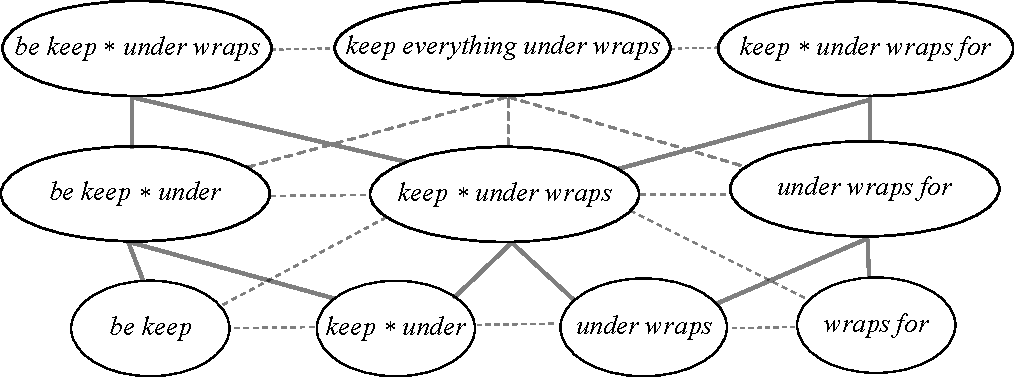
\includegraphics[width=0.8\textwidth]{FS_diagram_2.pdf}}
\caption{A portion of an $n$-gram lattice. Solid lines indicate subsumption, dotted lines overlaps}
\label{fig:example}
\end{figure*}

\subsection{Node interactions}

\subsubsection{Covering}

The most important node interaction is \termdef{covering}, which corresponds to discounting or entirely excluding a node based on the presence of a node higher in the lattice. Our model includes two types of covering: hard and soft. \termdef{Hard covering} is based on the idea that, due to very similar counts, we can reasonably conclude that the presence of $n$-gram in our statistics is a direct result of the other: if we have 143 counts of \ex{keep \gap under wraps} and 152 counts of \ex{under wraps}, the presence of \ex{keep \gap under wraps} almost completely explains \ex{under wraps}, and it is better if we collapse these two decisions into one. We do this by permanently disabling any covered node, and setting the the minLPR of the covering node to the maximum minLPR among all the nodes it covers, (including itself); this means that longer $n$-grams with function words (which often have lower minLPR) can benefit from the strong statistical relationships between open-class lexical features in $n$-grams that they cover. This is done as a preprocessing step, and so it greatly improves the tractability of the iterative optimization of the lattice. Of course, a threshold for hard covering must be chosen: empirically, we have found that a ratio of $2/3$ (corresponding to a significant but not overwhelming majority of the counts of a lower node corresponding to the higher node) works well.  We also use the concept of hard covering to address the issue of pronouns: due to pragmatic biases, pronouns often have higher than desirable LPR ratios \cite{Brooke15b}. In the lattice, $n$-grams with pronouns are considered covered (inactive) unless they cover at least one other node which does not have a pronoun, which allows us to greatly limit FS with pronouns without excluding them entirely: they are included only in cases where they are almost completely predictable from the context. 

%Another source of error are somewhat flexible FS which fall below our $n$-gram threshold but where some portion of the FS is above the threshold: to address this, we collect additional statistics and remove as a post-processing step any FS which are hard covered by an $n$-gram not in our lattice. 

\termdef{Soft covering} is used in cases when a single $n$-gram does not entirely account for another, but a turned-on $n$-gram to some extent may explain some of the statistical irregularity of one lower in the lattice. For instance, in \figref{fig:example} \ex{keep \gap under} is not hard-covered by \ex{keep \gap under wraps} (since there are FS such as \ex{keep \gap under surveillance}, \ex{keep it under your hat}, \etc), but if \ex{keep \gap under wraps} is tagged as an FS, we nevertheless want to discount the portion of the \ex{keep \gap under} counts that corresponds to occurrences of \ex{keep \gap under wraps}. This is accomplished by lowering the turned-off cost function of \ex{keep \gap under} (and thus making turning on less desirable) in the following manner: let $c(\dot)$ be the count function,and $s_1\dotts s_m$ be any turned-on nodes which are above $t$ in the lattice (covering nodes). Then, then the $d_0$ for a covered node $t$ is:

\begin{displaymath}
d_{0}(t) = \frac{c(t) - \sum_{i=1}^{m}{c(s_i)}}{c(t)}
\end{displaymath}

\noindent
This equation is intended as a simple, quick-to-calculate approximation of the result of recalculating minLPR with the counts corresponding to the covering nodes actually removed.

\subsubsection{Clearing}

In general, covering prefers turning on longer, covering $n$-grams since doing so lowers the turned-off cost function of nodes lower in the lattice. Not surprisingly, it is generally desirable to have a mechanism working in opposition, \ie one which generally prefers shorter $n$-grams. \termdef{Clearing} does this by changing the $C_0$ of nodes higher in the lattice when a lower node is turned-on. The basic mechanism is similar to covering, except that counts cannot be made use of in the same way; whereas it makes sense to discount the turned-off cost of covered nodes in proportion to the counts of their covering nodes (since the counts of the covered $n$-grams are due to the covering $n$-gram), in the reverse direction this logic fails. A simple but effective solution which avoids introducing parameters makes use of the minLPR values of the relevant nodes. In the most common (two node) situation, we lower the  $C_{0}(t)$ of the higher node according to the ratio between the minLPR of two nodes, though only if the minLPR of the lower node is higher. Generalized to consider the (rare) case of multiple clearing nodes, this is:

%in this paper, we consider two options: a hard clearing where any turned-on node will clear (set $C_{0}$ to 0 for) any node higher in the lattice which has a minLPR that is lower than it; and a soft 

\begin{displaymath}
C_{0}'(t) = max(1, C_{0}(t) \frac{minLPR(t)}{\prod{minLPR(s_i)})}
\end{displaymath}
where $s_i$ is the $i$th clearing node. We refer to this mechanism as clearing because it tends to clear away a variety of trivial uses of common FS which many have higher LPR due to the lexical and syntactic specificity of the FS. To give an example of its effect, if the node \ex{keep \gap under wraps} in \figref{fig:example} is turned on and has a minLPR of 8, then, if the minLPR of a node such as\ex{keep \gap under wraps for} is 4, the $C_{0}$ will be lowered to 2 ($4/(8/4)$) by clearing. This dissuades (but does not prevent) the model from turning on these nodes. Note that the effect of both covering and clearing is to lower the cost function for covered/clears nodes, which encourages the model to turn an $n$-gram like \ex{keep \gap under wraps} on, even supposing its minLPR were relatively low.

\subsubsection{Overlap}

The third mechanism of node interaction involves $n$-grams which overlap in the corpus. Though there are some exceptions, it is generally the case that independent formulaic sequences do not overlap. For example, given that \ex{be keep \gap under} and \ex{keep \gap under wraps} often appear together, overlapping on the tokens \ex{keep \gap under}, we do not want both being selected as an FS, even in the case where both had high minLPR. To address this problem, we use a mechanism somewhat different than above: rather than lowering the off-cost, we raise the on-cost. The idea behind lowering the cost when covering and clearing is to encourage the model to turn on nodes which effectively explain the presence of nodes above and/or below it in the lattice, but we do not want to encourage nodes that just happen to overlap with others; a penalty is a more appropriate mechanism. Let $oc(x,y)$ refer to number of times the $n$-grams corresponding to nodes $x$ and $y$ overlapped in the corpus, and $o_1\dotts o_m$ refer to \termemph{turned-on} nodes which overlap with our target node $t$. We define an $d_1$ exponential term for the $C_1$ our target node $t$ as:

\begin{displaymath}
d_{1}(t) = \frac{c(t)}{c(t) - \sum_{i=1}^{m}{oc(o_i)}}
\end{displaymath}

The effect of overlaps on the cost is hyperbolic: small amounts of overlapping has little effect, but with significant overlap the cost becomes prohibitive, effectively forcing one of nodes to turn off. 

 
\subsection{Optimization}

The dependence of the cost functions of nodes on their neighbors as discussed in the preceding section effectively prohibit a global optimization of the lattice. Fortunately, though a majority of nodes in the lattice are connected to each other though some path, most of the effects of nodes on each other are relatively local, and effective local optimizations can be made tractable by applying some simple restrictions. The main optimization loop consists of iterations over the lattice until complete convergence (no changes in the final iteration). For each iteration over the main loop, each potentially active node is examined in order to evaluate whether its current status is optimal given the current state of the lattice. The order that we do this has an effect on the result: among the obvious options, good results are obtained when ordering nodes by frequency, which gives an implicit advantage to relatively common $n$-grams, since they will tend to be turned on first.

%The algorithm for optimization procedure is given in Figure X (???). 

Given the relationships between nodes that we have defined above, it is obviously not sufficient to consider switching only the present node; If, for instance, one or more of \ex{be keep \gap under wraps}, \ex{under wraps}, or \ex{be keep \gap under} has been turned on, the covering, blocking, or overlapping effects of these other nodes will likely prevent a competing node like \ex{keep \gap under wraps} from being correctly activated. Instead, the algorithm identifies a small set of nodes (relevant nodes) which are the most important to status of the node under consideration whose status should be considered simultaneously. Since turned-off nodes have no direct effect on each other, only turned-on nodes above, below, or overlapping with the current node need be considered.  Once the relevant nodes have been identified, all nodes (including turned-off nodes) whose cost function is affected by one or more of the relevant nodes are identified, and then a greedy search is carried out for the optimal configuration of the relevant nodes starting from an `all-on' state. 

In practice, we apply the following restrictions which significantly reduce the runtime of the algorithm without sacrificing the quality of the output lexicon (based on development set testing):

\begin{itemize}
\item The complexity of the algorithm increases exponentially with the number of relevant nodes, so we limit the total number to 5. When there are more than 5 nodes turned on in the vicinity of the target node, relevant nodes are selected by ranking in terms of the influence of the nodes on each other as given by the relative change in their cost functions.
\item The full set of pairwise $n$-gram overlaps in a large corpus is too big too effectively store, and so we exclude overlaps with a count of less than 5 from our lattice.
\item Many nodes have a minLPR which is a little larger than 1. There is very little chance these nodes will be activated by the algorithm, and so after applying hard covering we do not consider activating nodes with a minLPR of less than 2.
\end{itemize}

\begin{table*}[!bt]
 
 \begin{center}
  \caption{ Statistics for test sets}
	 \label{tab:stats}
	 \begin{tabular}{lccccc}

       \hline
			& Contiguous FS & Contiguous non-FS & Gapped FS & Gapped non-FS & Fleiss Kappa\\
			 \hline
			ICWSM & 169 & 702 & 29 & 916& 0.84 \\
			BNC & 33 & 395 & 7 & 474 & 0.75 \\
			Croatian & 64 & 382 & 11 & 456 & 0.87 \\
			Japanese & 124 & 286 & 36 & 341 & 0.81\\
       \hline
 \end{tabular}

 \end{center}

 \end{table*}	

\section{Evaluation} \label{sec:evaluation}

We evaluate our approach across three different languages including evaluation sets derived from four different corpora. In English, we follow Brooke et \al \shortcite{Brooke15b} in using a 890M token filtered portion of the ICWSM social media corpus \cite{ICWSM} tagged with the Tree Tagger \cite{Schmid95}. To facilitate a comparison with Newman et \al \shortcite{Newman12}, which does not scale up to a corpus as large as the ICWSM, we also build a lexicon using the 100M token British National Corpus \cite{BNC}, using the standard CLAWS-derived POS tags for the corpus. Lemmatization included removing all inflectional marking from both words and POS tags. For English, we took the same POS regex used in Brooke et \al \shortcite{Brooke15b}, which includes simple nouns and portions thereof, up to a maximum length of 4.

The other two languages we include in our evaluation are Croatian and Japanese. Relative to English, both languages are free-word order: we were interested in probing the challenges associated with using an $n$-gram approach to FS extraction in such languages. For Croatian, we used the X corpus, a collection of X. The POS regex for Croatian included XXX. .... For Japanese we used a portion of the X corpus of roughly the same size (by token) as the ICWSM. The POS regex for Japanese...

Brooke et \al \shortcite{Brooke15b} introduced a method for evaluating formulaic sequence extraction without a reference lexicon or direct annotation of the output of a model: instead, $n$-grams are sampled after applying the frequency threshold and annotated as being either an FS or not, allowing for calculation of a true F-score for any model. We use the annotation of 2000 $n$-grams in the ICWSM corpus from that earlier work, and applied the same annotation methodology to the other corpora discussed above: based on written guidelines derived from the definitions of Wray \cite{Wray08} and at least one practice round,three native-speaker, educated annotators judged 500 contiguous $n$-grams and another 500 gapped $n$-grams for each of the new corpora. 

Other than the inclusion of new languages, our test sets differ from Brooke et \al \shortcite{Brooke15b} in two ways. First, instead of relying on strict majority annotation, we entirely excluded $n$-grams which just one annotator marked as FS. One advantage of a type-based annotation approach (as compared to a corpus annotation), particularly with regards to an task with a known subjective component, is that it is quite sensible to simply discard borderline cases, improving the reliability of evaluation at the cost of some representativeness.  Second, for the main evaluation we collapsed gapped and contiguous $n$-grams into a single test set. The rationale is that the number of positive gapped examples was too low (particularly for the BNC and the Croatian corpus) to provide a reliable independent F-score (see further of discussion of gapped phrases in \secref{sec:discussion}). Statistics for the four test sets are given in \tabref{tab:stats}.



% For these test sets, we report (in Table 1) inter-annotator agreement in terms of average $f$-score across annotators, which is appropriate for highly-imbalanced class situations such as this (formulaic is considered the positive class for this and other calculations), and also provides a human upper bound. 

%In addition, we also test the ICWSM-derived lexicon against the ``MWE'' test set from Brooke et \al \shortcite{Brooke15b} whose $n$-gram annotations (both gappy and non-gappy) are derived from the MWE annotation of Schneider \shortcite{Schneider14b}.

Our primary comparison is with the heuristic LPR model from Brooke et \al \shortcite{Brooke15b}. For the BNC, we also compare, separately, the DP-seg model from Newman et \al \shortcite{Newman12}: because the latter only handles sequential output, we use only the sequential part of the BNC test set. Both these models have been compared against a wide range of association measures;\footnote{One popular association measure which is theoretically extensible to $n$-grams of any length but which has not been addressed in the context of unrestricted MWE/FS identification is the (log-)likelihood ratio \cite{Dunning93}. Calculating a likelihood ratio in the general case involves considering all possible ways an $n$-gram could have been generated statistically from its component words: that is, whereas minLPR only considers the addition of one word to each $n-1$-gram, likelihood ratios must consider all combinations of all component $n-1,2,3\ldots$-grams, including, in our case, not only contiguous but also non-contiguous components. The corresponding exponential increase in complexity renders it and other such methods impractical for unrestricted FS identification.} we do not repeat all these comparisons here, but we do consider a lexicon built from ranking $n$-grams according to the measure used in our lattice (minLPR) as well as PMI. For each of these two association measures we build a lexicon equal to the size of the lexicon produced by our model. All comparisons here are subject to the same $n$-gram frequency threshold as the main model, since the content of our test sets are also linked to this threshold.

We created small development sets for each corpus and used them to do a thorough testing of parameter settings and other options, many of which we have excluded from our discussion here. Although it is generally possible to increase precision by increasing $C$, we found that across corpora we were always obtained near-optimal results using a $C$ of 4, so to demonstrate the usefulness of the lattice technique as an entirely off-the-shelf tool, we present the results using identical settings for all 4 corpora. We treat covering as a fundamental part of the Lattice model, but to investigate the efficacy of other node interactions within the model we present results with each of overlap and clearing node interactions turned off.

 \begin{table*}[!bt]
 
 \begin{center}
  \caption{ Results of formulaic sequence identification in various test sets; PMIrank = lexicon created by ranking pointwise mutual information, minLPRrank = lexicon created by ranking minLPR, LPRseg = lexicon created by method of Brooke at \al (2015), -cl = no clearing, -ovr = no penalization of overlaps, P = Precision, R = Recall, F = F-score. Bold is best in column.}
	 \label{tab:main}
 \begin{tabular}{lcccccccccccccccc}

       \hline
        \hline
				& \multicolumn{7}{c}{\bf{English}} & & \multicolumn{3}{c}{\bf{Croatian}} & & \multicolumn{3}{c}{\bf{Japanese}} \\
       \cline{2-9}			
       & \multicolumn{3}{c}{\bf{ICWSM}} & &  \multicolumn{3}{c}{\bf{BNC}} & & &&&  && & \\
       \cline{2-4} \cline{6-8} \cline{10-12} \cline{14-16}
           \multicolumn{1}{c}{\bf{Source}}    & P & R & F &   & P & R & F &   & P & R & F &  & P & R & F \\
            \hline
           \hline     
           
PMIrank & 0.24& 0.15& 0.18 & & 0.12 & 0.24 & 0.16 & & 0.21 &0.32 & 0.26 & & 0.23& 0.09 & 0.15 \\ 
minLPRrank & 0.49& 0.31 & 0.39 & & 0.25& 0.45 & 0.32 & & 0.36 & 0.45 & 0.40 &  & 0.51 & 0.14 & 0.22 \\ 

LPR-seg  &0.53 & 0.42 & 0.47 && 0.38 & 0.44 & 0.41 & & 0.41 & 0.47  & 0.43 &  & 0.77 & 0.34 & 0.47 \\ 
  \hline 

	Lattice \emph{-cl} & 0.57& 0.42 & 0.49 & & 0.34& 0.59 & 0.43 & & 0.39 & 0.56 & 0.46 & & 0.74 & 0.39 & 0.51 \\  	 
			
	Lattice \emph{-ovr} & 0.52& \bf{0.53} & 0.53 & & 0.34& \bf{0.60} & 0.43& & 0.35 & \bf{0.65} & 0.45 & & 0.69 & \bf{0.51} & \bf{0.59} \\  
			
				Lattice & \bf{0.67} & 0.45 & \bf{0.54} & & \bf{0.39}& 0.59 & \bf{0.47} & &\bf{0.42} & 0.57 & \bf{0.48} & & \bf{0.86} & 0.39 & 0.54 \\ 
            \hline
           \hline                  

 \end{tabular}

 \end{center}


 \end{table*}


 \begin{table}[!bt]
 
 \begin{center}
  \caption{ Results of formulaic sequence identification in sequential BNC test set; DP-seg = method of Newman et \al (2012)}
	\label{tab:BNC}
	
	 \begin{tabular}{lccc}

       \hline
			& P & R & F\\
			 \hline
			minLPRrank & 0.34 & 0.45 & 0.39 \\
			LPR-seg & 0.42 & 0.45 & 0.43 \\
			DP-seg & 0.34 & 0.71 & 0.46 \\
			Lattice & 0.46 & 0.61 & 0.53 \\
       \hline
 \end{tabular}

 \end{center}

 \end{table}			

\section{Results}

The main results for FS acquisition across all four corpora are shown in \tabref{tab:main}. As noted in previous work, simple statistical association measures like PMI do fairly poorly when faced with unrestricted $n$-grams of variable length: minLPR is clearly a much better statistic for this purpose. The LPRseg method of Brooke et \al \shortcite{Brooke15b} consistently outperforms simple ranking, and the lattice method proposed here does better still, with a margin that is fairly consistently across languages, though the margin is slightly larger for English corpora. Generally, using clearing and overlap node interactions offer an relatively large increase in precision at the cost of a smaller drop in recall, though the change is fairly symmetrical with in Croatian, and in Japanese precision is already high enough relative to recall that the f-score is not improved. The ICWSM corpus also has relatively high precision, whereas both the BNC and Croatian corpus have low precision and high recall.

In the continuous FS test set for the BNC (\tabref{tab:BNC}), we found that the DP-seg method of Newman \cite{Newman12} was also able to beat our baseline methods, but with regards to F-score, it was inferior to our Lattice method. Some of that difference seems attributable to a severe precision/recall imbalance, though it was one we unable to improve by changing the parameters of the model from recommended settings.


			
\section{Discussion} \label{sec:discussion}

Though the results across the four corpora are reasonably similar with respect to overall f-score, there are a significant discrepancies. By using the UniDict morpheme representation for Japanese, the model is, in essence, doing an extra layer of FS identification, one which is provided by word boundaries in the other languages. The result is that there are many more FS for Japanese. Precision is very high, and recall is relatively low. Under these conditions, methods which tend to increase precision at the cost of recall will be less desirable with respect to f-score, which explains why the full model is not the best in that case.  Importantly, the initial $n$-gram statistics derived from corpus reflect that Japanese is different: the number of $n$-gram types over length 4 is almost twice the number in the ICWSM, or almost 14\% of all $n$-gram types. One idea for future work is to automatically adapt to the particular properties of the input language/corpus, though it might also be worth considering whether f-score is the most appropriate metric, given that high precision seems particularly desirable in a lexical resource.

At the opposite end of the precision/recall curve, the low precision of the BNC is almost certainly at least somewhat a reflection of its relatively low size: whereas the $n$-gram threshold we have used here results in a minimum counts of in the order of about 100 for the other three corpora used here, the BNC statistics includes $n$-grams which appear less than 10 times. This might be resolved, of course, by increasing the $n$-gram threshold, or simply avoiding small corpora altogether, but it may be useful to focus effort on how to building comprehensive FS lexicons even in relatively low resource situations. One idea we are actively pursing is modifying the calculation of the LPR metric to integrating uncertainty due to low counts.

There is one another more general explanation for the precision/recall imbalances we see across the four corpora: Both the BNC and the Croatian corpus are composed primarily (though not exclusively) of published texts written by professional writers, in particularly newswire. The ICWSM and the Japanese corpus, on the other hand, are mostly blogs and other internet genres. Though all genres have FS, there is much more diversity in less controlled genres: many English gapped expressions, in particular, are used almost exclusively in relatively informal genres. The fact that last than 20\% of the FS derived from the BNC appear in the lexicon for the ICWSM is fairly telling of how important genre differences are to the range of FS that will be seen in a particular corpus.

We were interested in addressing Croatian and Japanese in part because of their tendency towards relatively free word order, and whether allowing gaps in our FS would help with these languages. We discovered however, that free word order actually results in \emph{more} of a tendancy towards contiguous FS rather than less. Strikingly rare in Croatian (and to a lesser extent, Japanese), are expressions where the content of a gap is an argument which must be filled to syntactically complete an expression: it is the relatively fixed-order of English that sometimes keeps elements of an FS distant from each other in order to satisfy fixed-word-order constraints. The gaps that do happen in Croatian are mostly prosody-driven insertions of other elements into already complete FS. This phenomena actually highlights a problem with the model, in that gapped and contiguous version of the same $n$-gram sequence are, at present, considered entirely independently. Alternatives for dealing with this range from collapsing statistics to create a single node, or linking contiguous and gapped versions of the same $n$-grams sequence in the lattice model, encouraging them to have the same FS labels.

A third, more ambitious option would be to switch to a dependency representation. This option actually requires very little change to the model presented here, since all the basic relationships in the lattice as well as the LPR metric could be straightforwardly defined in terms of subgraphs instead of strings. One clear negative is the need for a dependency parser for the language and domain of interest, and that there is no potential for the use of FS to improve parsing. A most subtle issue is that switching to a dependency representation does not entirely eliminate the need for syntactic gaps in order to represent a full range of FS: there are a small category of gappy FS where the gap term actually forms the syntactic connection between the two parts of the expression, \ie \ex{no amount of * can}.

As it stands, connections in the lattice are based entirely on explicit $n$-gram subsumption and overlap relations. Another connection could be based on identical or similar syntactic patterns (\eg POS sequences), which could serve to encourage the model to make generalizations: in English, for instance, learning that verb-particle constructions are generally likely to be FS. Our investigations thus far suggest that it may be difficult to apply this idea without merely amplifying existing biases in the LPR measure. Bringing in other information, for instance some simple distributional statistics which might help us identify which $n$-grams have non-compositional semantics, would, could, in combination with the existing lattice competition, help us focus the model on detecting MWEs, which could then serve as a reliable basis for generalizing to $n$-gram for which the raw LPR statistics are an unreliable indicator.

Finally, though in general using the sampling methodology to build test sets has significant benefits in terms of providing a robust, replicable evaluation, since precision and recall are both dependent on the number of positive examples, f-scores are unreliable when there are few positive examples. To do a independent evaluation of FS with gaps, we would want many more examples than can be produced with straightforward sampling. One option we could consider is a adding additional filtering to the sampling processes (\eg using the LPR metric to exclude large numbers of extremely poor $n$-grams), though it is difficult to do this without hopelessly biasing the evaluation, both in terms of the specific $n$-grams evaluated as well as the ratio between positive and negative examples. 





%Otherwise, gaps in MWEs have generally addressed by using full syntactic representations \cite{Seretan11}.
%One more restriction is necessary to make the use of overlaps feasible: without any restrictions, the number of connections resulting from overlaps is too large. We resolved this problem by excluding as possible active nodes. 

%a separate analysis of the that corpus showed the contents of most gapped FS in English were simple nouns or some portion thereof; this is somewhat less true for the more free word-order langauges we are also considering, but still a usuable heuristic. 

%which be described by the following (Penn Treebank) POS regular expression:

%\vspace{3mm}
%\noindent
% PP$\,$|$\,$[(PDT)(DT)JJ*[NN$\,$|$\,$NP]*(POS$\,$|$\,$PP\$)JJ*NN*]
%\vspace{1mm}

%(Our POS tags are given by the TreeTagger)

% For our main evaluation in English, our corpus is a 890 million version of the tier 1 texts in the ICWSM 2009 blog corpus \cite{ICWSM} which has been filtered to remove duplicates and near duplicates.
\bibliography{mybib}
\bibliographystyle{eacl2017}


\end{document}

%%% Local Variables:
%%% mode: latex
%%% TeX-master: t
%%% End:
